%% document class
\documentclass[10pt]{beamer}
%%theme
\usetheme[hideothersubsections,width=2cm]{Berkeley}
%% page settings
\usepackage{xcolor}
%%\usenavigationsymbolstemplate{}
\usefonttheme{structureitalicserif}
%%\defbeamertemplate*{footline}{shadow theme}

%% packages
\usepackage{courier}
\usepackage{geometry}
\usepackage{graphicx}
\usepackage[scaled=0.9]{helvet}
\usepackage{multimedia}
\usepackage{media9}
\usepackage{mathptmx}
\usepackage{tikz}
\usepackage{xmpmulti}
\usepackage{eso-pic}



%%color settings
%%%%% Color Schema
\definecolor{grey_dark}{RGB}{38,50,56}
\definecolor{grey}{RGB}{33,150,243}
\definecolor{gray_dark}{RGB}{39,36,41}
\definecolor{white}{RGB}{255,255,255}
\definecolor{orangish}{RGB}{255, 117, 26}
\definecolor{nvidia}{RGB}{116, 183, 27}
\definecolor{grey_light}{RGB}{242, 242, 242}

%% theme settings
\setbeamercolor*{palette primary}{fg=white,bg=grey_dark} % upper part
\setbeamercolor*{palette secondary}{fg=grey_dark,bg=nvidia} % left part (background)
\setbeamercolor*{sidebar left}{fg=white,bg=grey_dark} % left part with links
\setbeamercolor*{palette sidebar primary}{fg=nvidia}
\setbeamercolor*{palette sidebar secondary}{fg=white}
\setbeamercolor*{block title}{fg=grey_dark,bg=nvidia}
\setbeamercolor*{block body}{fg=grey_dark,bg=grey_light}
\setbeamercolor{section in toc}{fg=grey_dark}
\setbeamercolor{section number projected}{bg=nvidia}
\setbeamercolor*{item}{fg=nvidia} % bullets
\setbeamerfont{section in sidebar}{size=\scriptsize}

%% new commands
%\input{settings/macros}
\addtobeamertemplate{frametitle}{\vskip+0.6ex}{}
\makeatletter
\beamer@headheight=2\baselineskip
\makeatother

%% slide numbers
\makeatletter
\setbeamertemplate{frametitle}{%
	\nointerlineskip%
	\vskip-\beamer@headheight%
	\vbox to \beamer@headheight{%
		\vfil
		\leftskip=-\beamer@leftmargin%
		\advance\leftskip by0.3cm%
		\rightskip=-\beamer@rightmargin%
		\advance\rightskip by0.3cm plus1fil%
		{\usebeamercolor[fg]{frametitle}
			\usebeamerfont{frametitle}\insertframetitle\hfill\insertframenumber\par}% added number
		{\usebeamercolor[fg]{framesubtitle}
			\usebeamerfont{framesubtitle}\insertframesubtitle\par}%
		\vbox{}%
		\vskip-1em%
		\vfil
	}%
}
\makeatother
\newcommand\AtPagemyUpperLeft[2]{\AtPageLowerLeft{%
\put(\LenToUnit{0.05\paperwidth},\LenToUnit{0.89\paperheight}){#1}}}
\AddToShipoutPictureFG{
	\AtPagemyUpperLeft{{
\includegraphics[width=0.8cm,keepaspectratio]{images/kgp_logo.png}}}
}
\begin{document}
\title{Detecting Diabetic Rtinopathy using Deep Learning}


%% Title Page
%% Contributors Page
{
	\usebackgroundtemplate{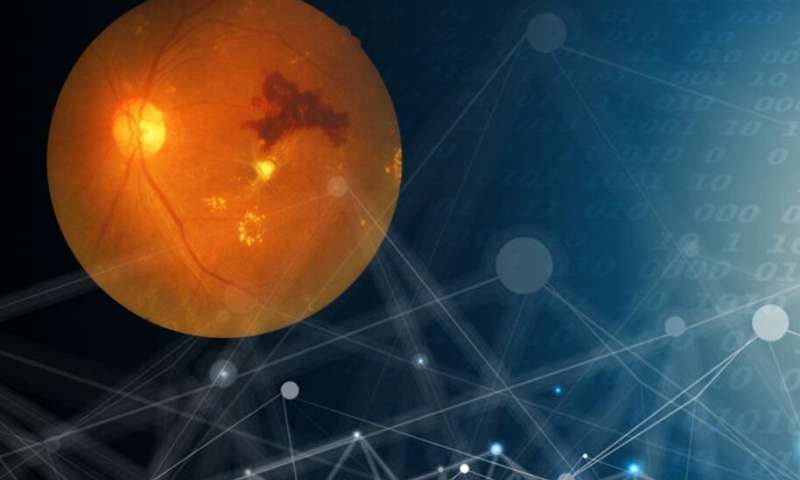
\includegraphics[height=\paperheight,width=\paperwidth]{images/DRDL}}
	\begin{frame}[plain]
		\titlepage
	\end{frame}
 	
}
\begingroup
\usebackgroundtemplate{%
	\tikz\node[opacity=0.3] {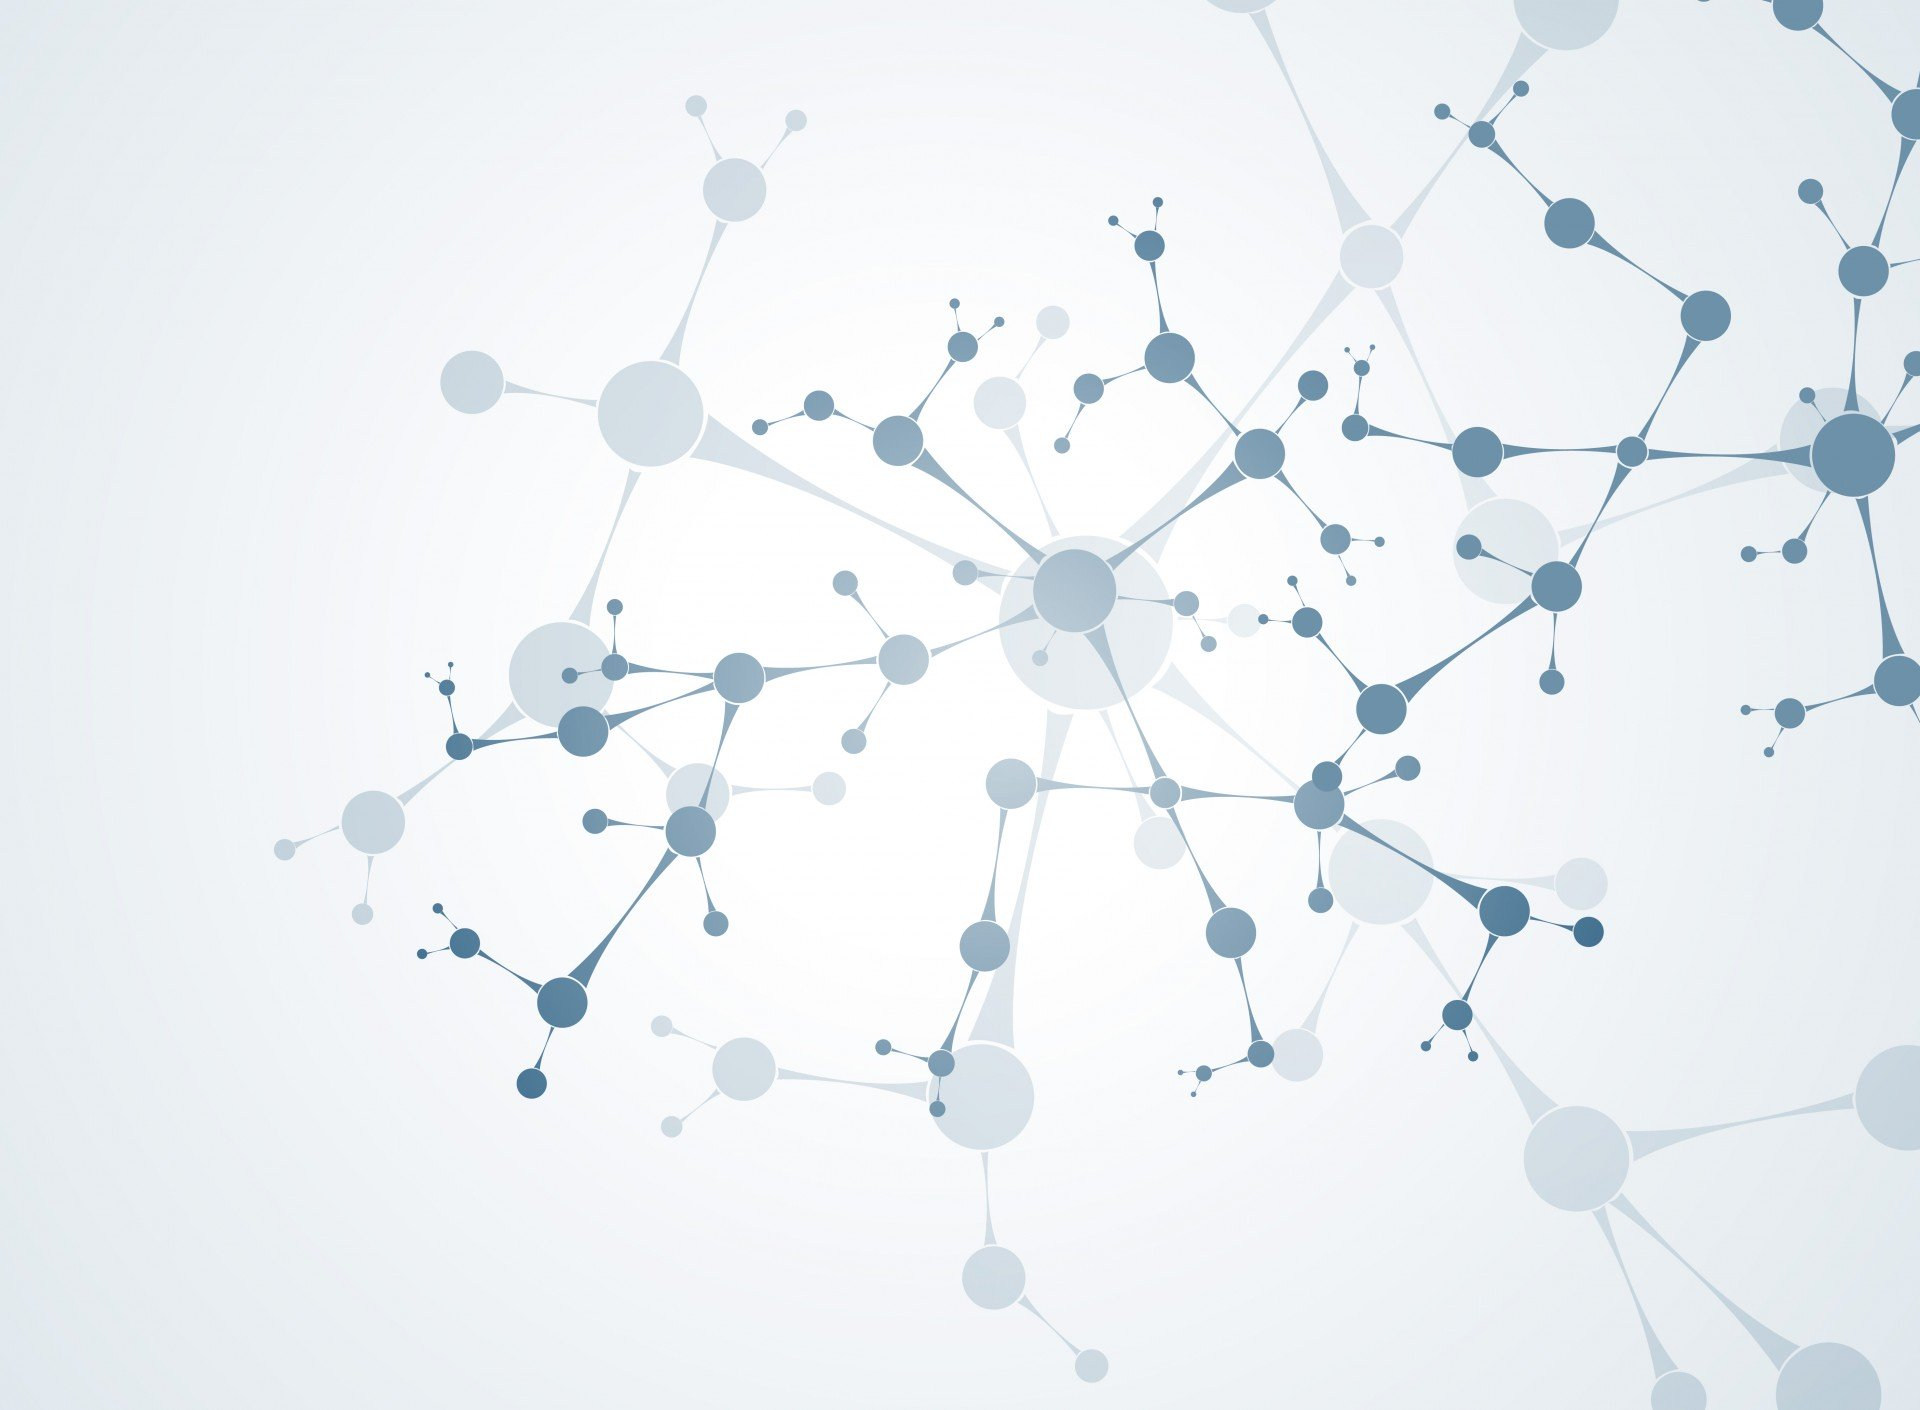
\includegraphics[height=\paperheight,width=\paperwidth]{images/bg-vec}}
	;}
	\begin{frame}[c]{Contributors}
		\begin{center}
			\Huge{Presented By:\\}
			\huge{~\\Subhajit Barh\\}
			\Large{~\\Department of Mathematics\\}
			\large{~\\(Computer Science and Data Processing)\\}
			\large{~\\Indian Institute of Technology Kharagpur\\}
		\end{center}
	\begin{center}
		
\includegraphics[width=1 cm,keepaspectratio]{images/kgp_logo.png}
	\end{center}
	\end{frame}
	%% contents
	\begin{frame}{Contents in Brief}
		%\tableofcontents
		\tableofcontents[hideallsubsections]
	\end{frame}
\endgroup
\begingroup
\usebackgroundtemplate{%
		\tikz\node[opacity=0.3] {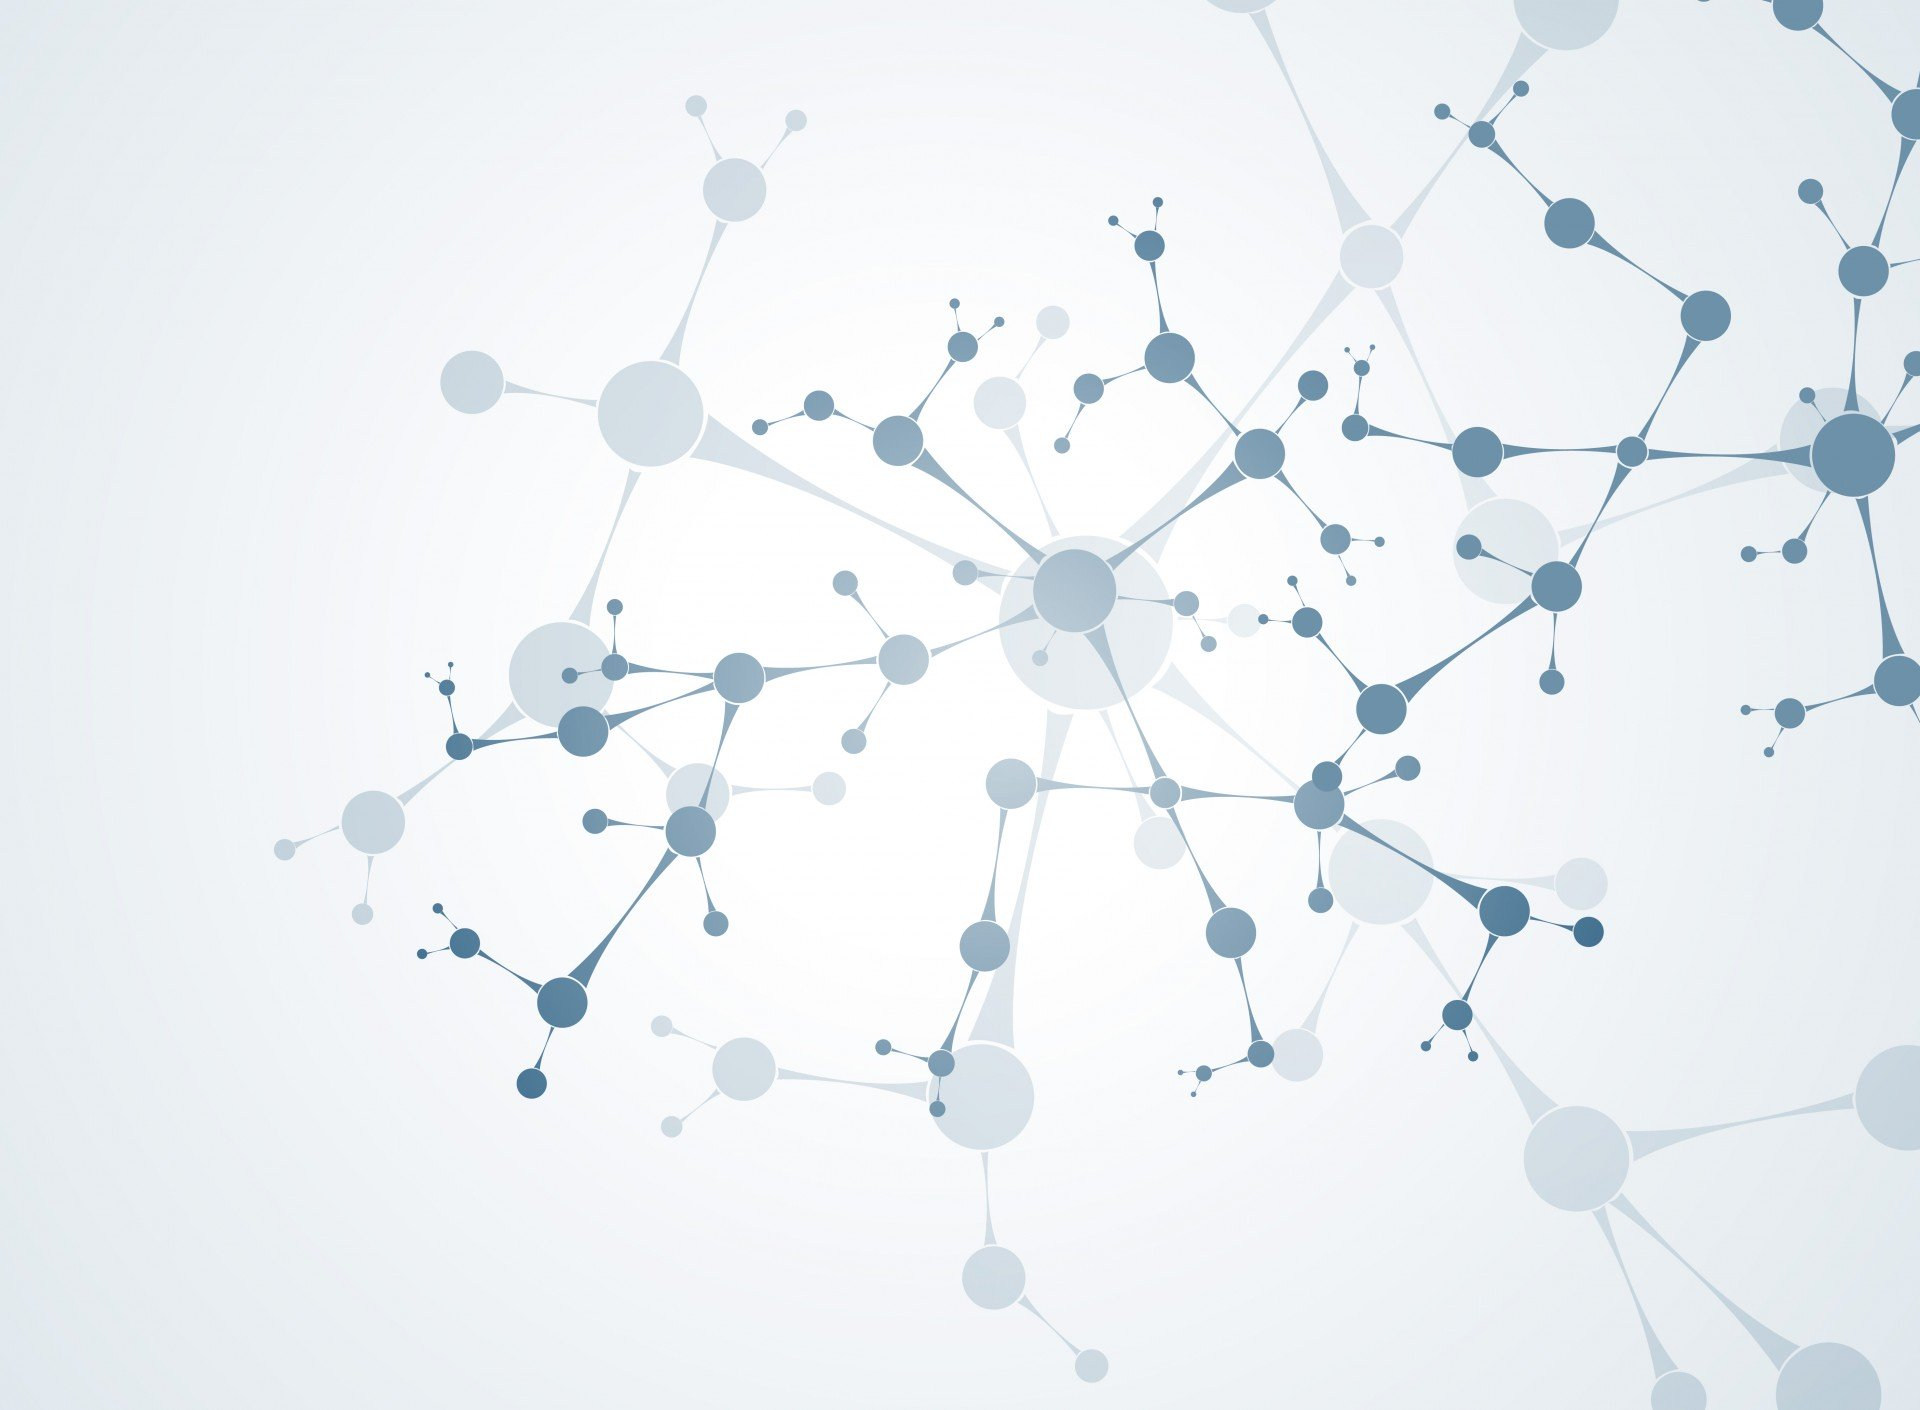
\includegraphics[height=\paperheight,width=\paperwidth]{images/bg-vec}}
		;}
	\section{Introduction}
		\subsection{What is DR}
			\begin{frame}{What is Diabetic Retinopathy?}
			Diabetic retinopathy (DR), also known as diabetic eye disease, is a medical condition in which damage occurs to the retina 					due to diabetes mellitus. It is a leading cause of blindness. Diabetic retinopathy affects up to 80 percent of those who have 			had diabetes aged 20 years or more. 
			\begin{figure}
				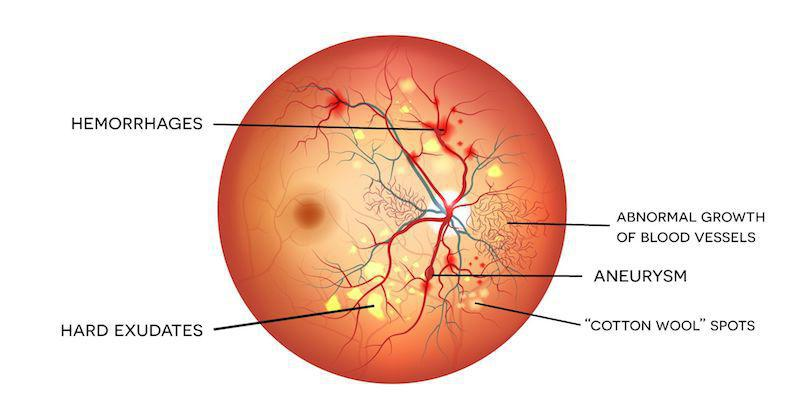
\includegraphics[width=\linewidth,height=2.5in]{images/DR}
			\end{figure}
			\end{frame}
			\begin{frame}{Types Of DR}
			Depending on severity we can devide Diabetic Retinopathy in 5 categories
			\begin{itemize}
			\item[0] - No DR

			\item[1]- Mild

			\item[2]- Moderate

			\item[3]- Severe

			\item[4]- Proliferative DR
			\end{itemize}
			
			\end{frame}
		
		\subsection{Detecting DR}
			\begin{frame}{Detecting Diabetic Retinopathy}
				\begin{block}{Manual Detection}
				Detecting Daiabetic Retinopathy is currently done by a method  called Dilated eye exam . In this method the doctor administers drops in patient's eye and take pictures of the retina. After reviewing  the image doctor have to manually conclude about the presence or advance of the disease . The doctor or experts generally looks for abnormalities in the blood vessels, optic nerve, retina,or formation of new blood vessels,retinal detachment,scar tissue etc .
				\end{block}\pause
				\begin{block}{Automated Detection}
				An automated tool for grading severity of diabetic retinopathy would be very useful for accerelating detection and treatment. We will use a Deep learning convolutional neural network model to detect Diabetic Retinopathy with minimum human intervention .
				\end{block}
			
			\end{frame}
		\subsection{Detecting DR using Deep Learning}
			\begin{frame}{Detecting DR using Deep Learning}
				We will use Convolutional Neural Network along with transfer Learning to detect and categorize the presence of diabetic Retinopathy 
			\end{frame}
	\section{Convolutional Neural Network}
		\subsection{What is CNN}
			\begin{frame}{What is Convolutional Neural Network}
				\begin{block}{CNN}
					CNN(convolutional Neural Network) is an neural network architecture which works really well with Images. Each 								Convolution Layer Consists of mainly three sub layers.
				\end{block}
				\begin{itemize}
					\item[1] Convolution layer
					\item[2] Pooling Layer
					\item[3] Fully Connected Layer
				\end{itemize}
			\end{frame}
			\begin{frame}{Convolution Layer}
				In convolution layer the filter(a smaller dimentional matrix) moves to the right with a certain Stride Value till it parses the complete width. Moving on, it hops down to the beginning (left) of the image with the same Stride Value and repeats the process until the entire image is traversed.In each step it computes the dot product with the original matrix and thus constructs the output matrix.
				\transduration<0-8>{0}
        		\multiinclude[<+->][format=png, graphics={width=\textwidth,height=5cm}]{images/cnn/cnn}
			\end{frame}
			\begin{frame}{Pooling Layer}
				Similar to the Convolutional Layer, the Pooling layer is responsible for reducing the spatial size of the Convolved Feature

There are two types of Pooling: Max Pooling and Average Pooling. Max Pooling returns the maximum value from the portion of the image covered by the Kernel. On the other hand, Average Pooling returns the average of all the values from the portion of the image covered by the Kernel
				\transduration<0-8>{0}
        		\multiinclude[<+->][format=png, graphics={width=\textwidth,height=5cm}]{images/Pooling/pooling}
			\end{frame}
			\begin{frame}{Fully Connected Layer}
			The fully connected layer is nothing but a ordinary perception based network. Here  we flattened our matrix into vector and feed it into a fully connected layer like any other neural network.
			\begin{figure}
				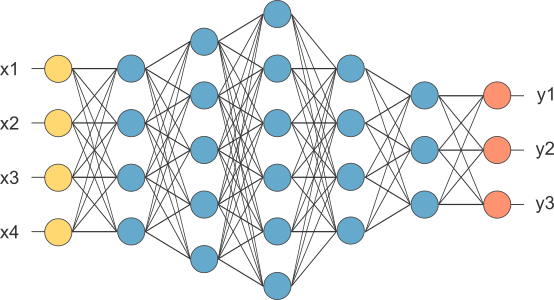
\includegraphics[width=\linewidth,height=2.5in]{images/fc}
			\end{figure}

			\end{frame}
		\subsection{Back Propagation}
			\begin{frame}{Back Propagation and Optimization}
			All those filters have weights. Those weights and percepton weights in FC layers must be learned using back-propagation .
			In each iteration we update those weights using our optimizer.Here we used Gradient Descent optimizer.But in future we can use optimizers like adam or adaguard etc.
			
			\end{frame}
			\subsection{Gradient Descent}
			\begin{frame}{Gradient Descent}
			\begin{block}{Gradient Descent}
			Gradient descent is a iterative optimization algorithm for finding the minimum of a function. To find a local minimum of a function using gradient descent, one takes steps proportional to the negative of the gradient (or approximate gradient) of the function at the current point
			\end{block}			
			\end{frame}
			\begin{frame}{Gradient Descent}
				Cost function or error function  can be an indicatior of how accurate our model is and optimizer uses that to optimize our model. Here we will use MSE loss. Which is defined as
				\begin{equation}
					J(w,b)=\dfrac{1}{M}\sum(h_{(w,b)}(x^{(i)})-y^{(i)})^2
				\end{equation}
				Then we calculate gradients of the cost function as below
				\begin{equation}
					\nabla_w J =\dfrac{\partial}{\partial{w}} J(w,b)
				\end{equation}
				\begin{equation}
				\nabla_b J=\dfrac{\partial}{\partial{b}} J(w,b)
				\end{equation}
				Then we update the weights using the formula as below
				\begin{equation}
				w{}'=w-\alpha \nabla_wJ
				\end{equation}
				\begin{equation}
					b{}'=b-\alpha \nabla_bJ
				\end{equation}
			\end{frame}
			\begin{frame}{Gradient Descent}
					\begin{figure}
					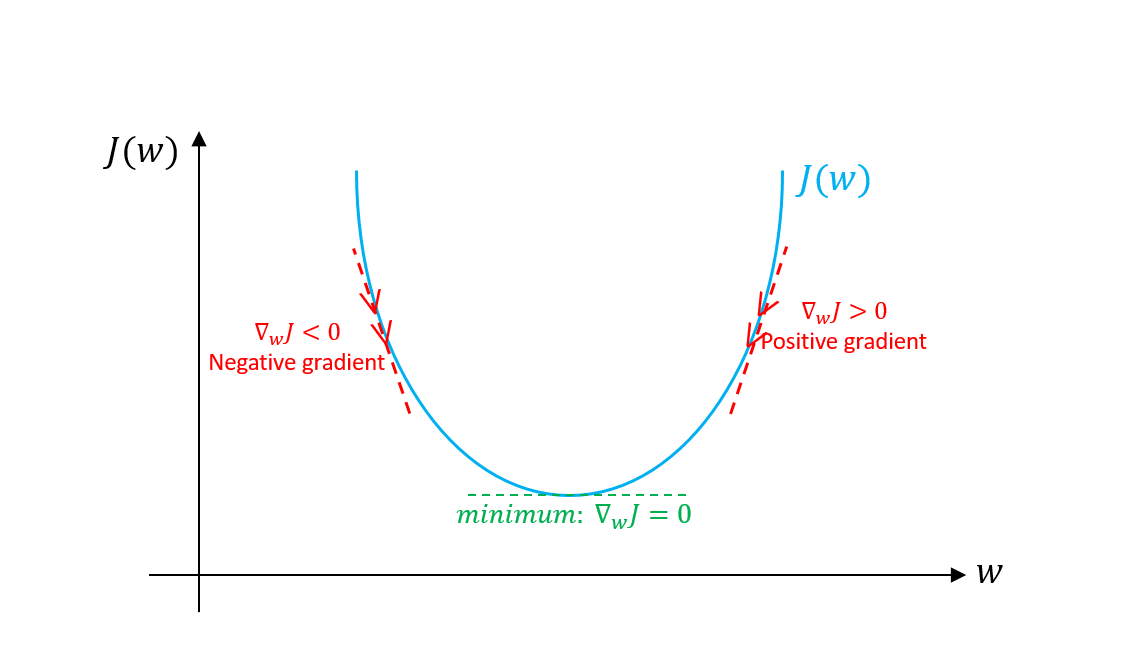
\includegraphics[width=10 cm,keepaspectratio]{images/graddec3}		
				\end{figure}
			\end{frame}				
							
			
	\section{Transfer Learning}
		\subsection{What is Transfer Learning}
			\begin{frame}{What is Transfer Learning}
				Transfer learning is a process in which we make use of the knowledge gained while solving one problem and applying it to a different but related problem .
			\end{frame}
		\subsection{Pretrained Models}
			\begin{frame}{Pretrained Models}
			Here we use a pre-trained big model named resnext101(~44 million parameters) which was trained by facebook on Imagenet .
We take the resnext101 model chop the last layer down and add our custom regression layer to classify the images.
			\end{frame}
		\section{Data}
		\begin{frame}{Data}
			Asia Pacific Tele-Ophthalmology Society (APTOS) and Aravind Eye Hospital of India published a dataset of retina images through Kaggle.The Data-set can be found on 
		\url{https://www.kaggle.com/c/aptos2019-blindness-detection/data}
		With quick exploration we can visualize the data as follows
		\begin{figure}
			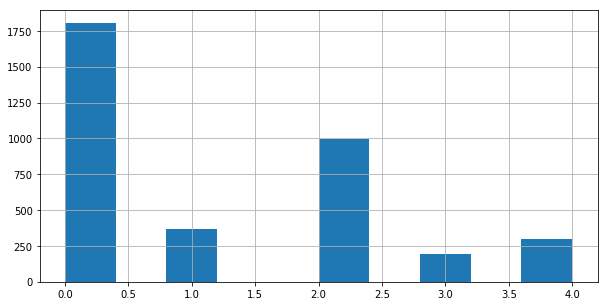
\includegraphics[width=\linewidth]{images/DataLabels.png}
		\end{figure}
		
		\end{frame}
	\section{Training and Finetuning}
		\subsection{Trainining}
			\begin{frame}[fragile]
			First we train the model freezing the base layers. we do this for 30 epochs
			we used
			\begin{itemize}
				\item[1]Gradient Descent  as Optimizer
				\item[2]learning rate=0.001
				\item[3]cost function is Mean Square Error
			\end{itemize}
			
			\end{frame}
		\subsection{FineTuning}
			\begin{frame}
				Then we fine Tune the whole model for another 30 epochs .Here we unfreeze the base layer
				\begin{itemize}
				\item[1]Gradient Descent  as Optimizer
				\item[2]learning rate=0.0001
				\item[3]cost function is Mean Square Error
			\end{itemize}
				
			\end{frame}
	\section{Result}
			\begin{frame}{version 7(loss graph)}
				\begin{figure}
					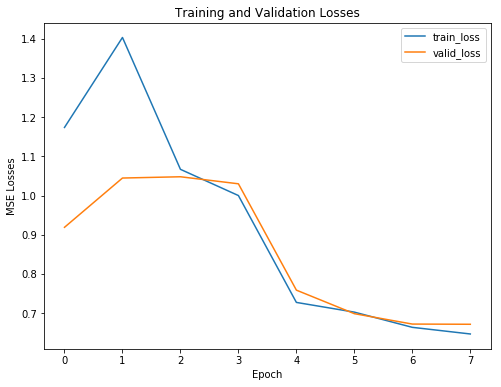
\includegraphics[scale=.5]{Results/v38lossgraph}
				\end{figure}
			\end{frame}
			\begin{frame}{version 7(Confusion Matrix)}
				\begin{figure}
					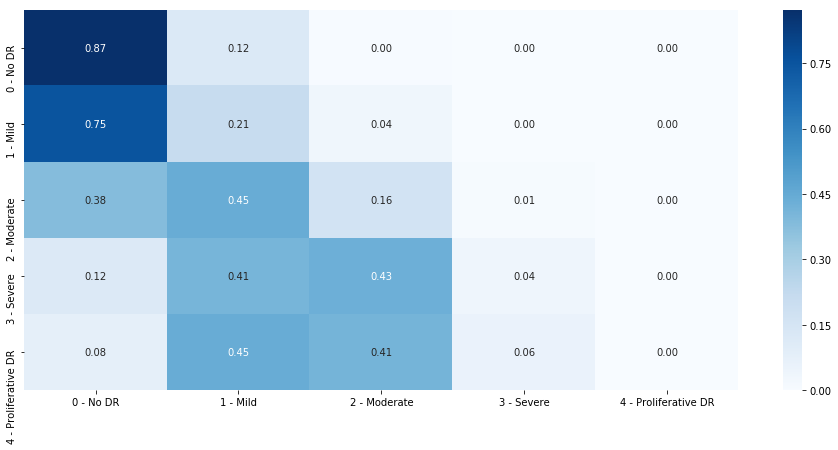
\includegraphics[width=\linewidth]{Results/v38confusion}
				\end{figure}
			\end{frame}
			\begin{frame}{version 49(loss graph)}
				\begin{figure}
					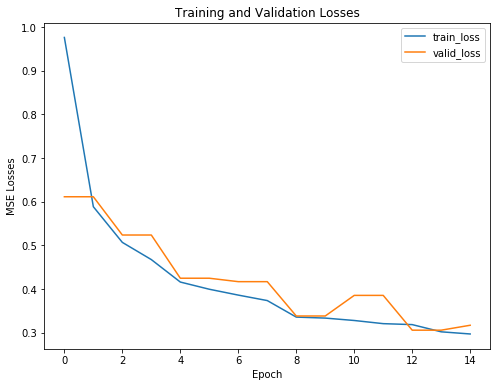
\includegraphics[scale=.5]{Results/v49lossgraph.png}
				\end{figure}
			\end{frame}
			\begin{frame}{version 49(Confusion Matrix)}
				\begin{figure}
					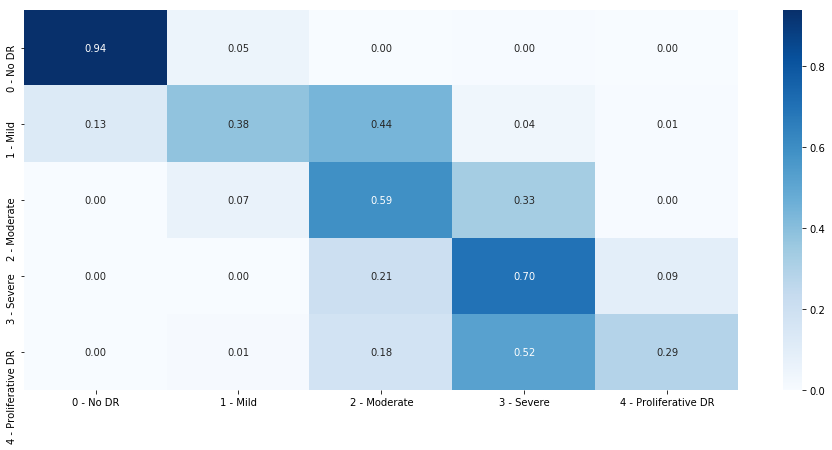
\includegraphics[width=\linewidth]{Results/v49wooptimizationconfusion.png}
				\end{figure}
			\end{frame}
			\begin{frame}{version 51(loss graph)}
				\begin{figure}
					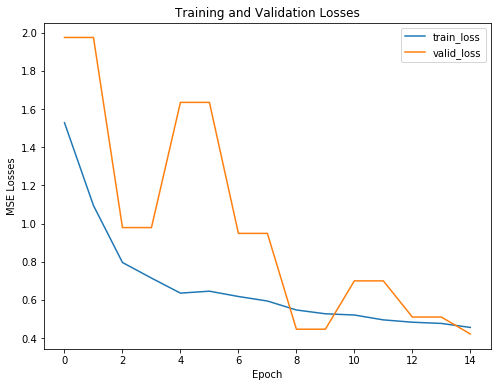
\includegraphics[scale=.5]{Results/v51lossgraph.png}
				\end{figure}
			\end{frame}
			\begin{frame}{version 51(Confusion Matrix)}
				\begin{figure}
					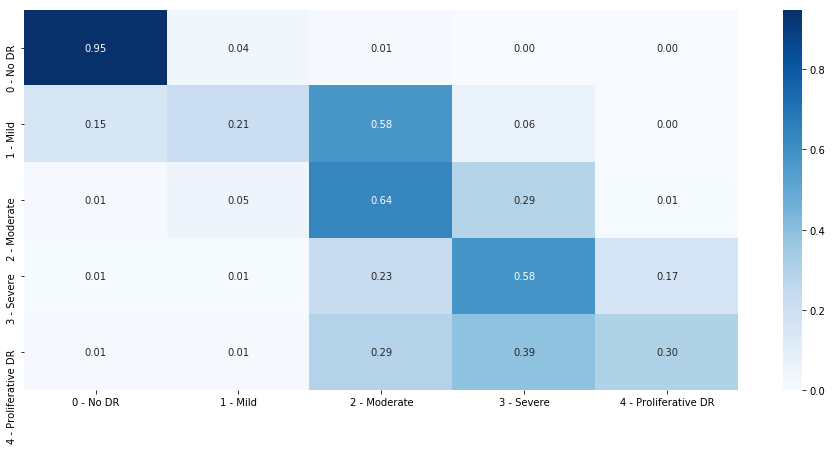
\includegraphics[width=\linewidth]{Results/v51confusionmatrix.png}
				\end{figure}
			\end{frame}
			\begin{frame}{version 23(Fine tuned loss graph)}
				\begin{figure}
					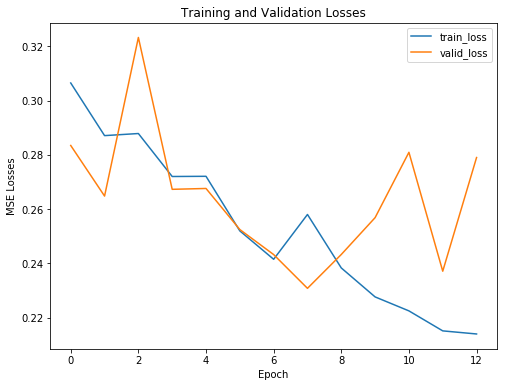
\includegraphics[scale=.5]{Results/vI23lossgraph.png}
				\end{figure}
			\end{frame}
			\begin{frame}{version 23(Fine tuned Confusion Matrix)}
				\begin{figure}
					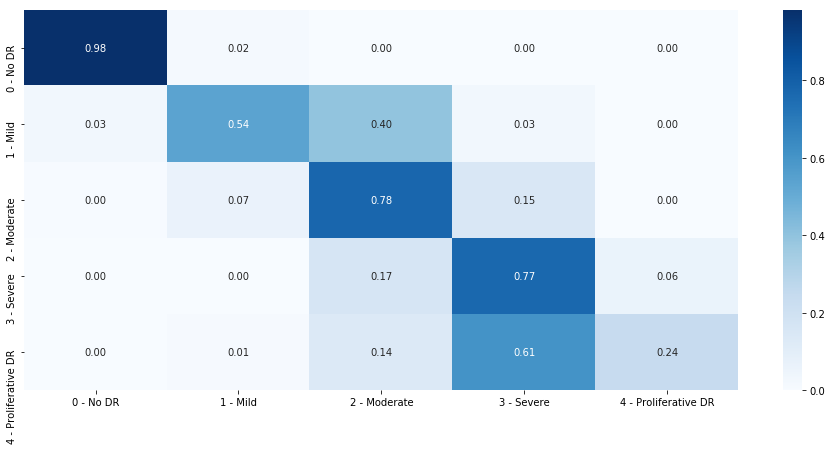
\includegraphics[width=\linewidth]{Results/VI23confusion.png}
				\end{figure}
			\end{frame}
			\begin{frame}{version 26(Fine tuned loss graph)}
				\begin{figure}
					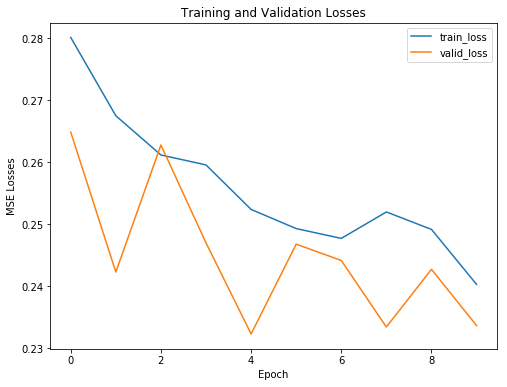
\includegraphics[scale=.5]{Results/vI26lossgraph.png}
				\end{figure}
			\end{frame}
			\begin{frame}{version 26(Fine tuned Confusion Matrix)}
				\begin{figure}
					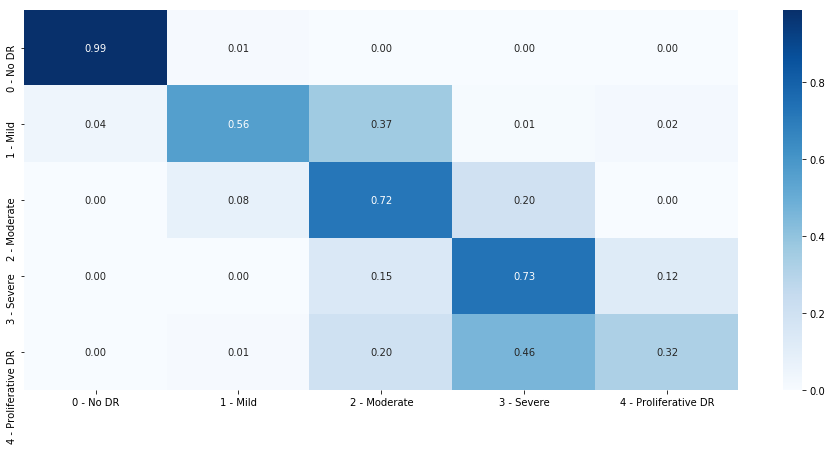
\includegraphics[width=\linewidth]{Results/VI26confusionmatrix.png}
				\end{figure}
			\end{frame}
	\section{Code}
		\begin{frame}{Code}
			Github Link:\url {}
			Kaggle Link: \url{https://www.kaggle.com/subhajitbarh/inference-model?scriptVersionId=18068811}
		\end{frame}				
	\section{Deficiency}
			\begin{frame}{Deficiency }
			\begin{center}
				\begin{itemize}
					\item[1)] This model is very slow .Without GPU it takes more than 5 minutes to predict single image \pause
					\item[2)] This model is very big .It is almost 2 GB in size.Which makes it impossible for Deployment  \pause
				\end{itemize}
			\end{center}
			\end{frame}
	\section{Improvement}
			\begin{frame}{Room for Future Improvements}
			\begin{center}
				\begin{itemize}
					\item[1)] for pre-trained model we can use something like efficient-net which is significantly smaller \pause
					\item[2)] We can use Heat-Map of model and overlay it on the top of existing picture to help human experts to conclude  \pause
				\end{itemize}
			\end{center}
			\end{frame}
	\section{References}
			\begin{frame}{References}
				\begin{enumerate}
					\item \textit{Preprocessing the Image} \url{https://www.kaggle.com/ratthachat/aptos-eye-preprocessing-in-diabetic-retinopathy} 
					\item \textit{Dataset} \url{https://www.kaggle.com/c/aptos2019-blindness-detection} 
					\item \textit{Gradient Descent} \url {https://towardsdatascience.com/understanding-the-mathematics-behind-gradient-descent-dde5dc9be06e} 
					\item \textit{Transfer Learning} \url {https://towardsdatascience.com/what-is-transfer-learning-8b1a0fa42b4} 
					\item \textit{ReNext} \url {https://github.com/facebookresearch/ResNeXt} 
					
				\end{enumerate}
			\end{frame}
		
\endgroup

\end{document}
